\documentclass{article}

\usepackage{fancyhdr}
\usepackage{lastpage}
\usepackage{extramarks}
\usepackage[usenames,dvipsnames]{color}
\usepackage{courier}
\usepackage{amsmath}
\usepackage{amsthm}
\usepackage{amsfonts}
\usepackage{tikz}

\usetikzlibrary{automata,positioning}

\topmargin=-0.45in
\evensidemargin=0in
\oddsidemargin=0in
\textwidth=6.5in
\textheight=9.0in
\headsep=0.25in

\linespread{1.1}

\pagestyle{fancy}
\lhead{\hmwkAuthorName}
\chead{\hmwkClass\ (\hmwkClassInstructor\ \hmwkClassTime): \hmwkTitle}
\rhead{\firstxmark}
\lfoot{\lastxmark}
\cfoot{}
\renewcommand\headrulewidth{0.4pt}
\renewcommand\footrulewidth{0.4pt}

\setlength\parindent{0pt}

\newcommand{\enterProblemHeader}[1]{
    \nobreak\extramarks{#1}{#1 continued on next page\ldots}\nobreak
    \nobreak\extramarks{#1 (continued)}{#1 continued on next page\ldots}\nobreak
}

\newcommand{\exitProblemHeader}[1]{
    \nobreak\extramarks{#1 (continued)}{#1 continued on next page\ldots}\nobreak
    \nobreak\extramarks{#1}{}\nobreak
}

\setcounter{secnumdepth}{0}
\newcounter{homeworkProblemCounter}

\newcommand{\homeworkProblemName}{}
\newenvironment{homeworkProblem}[1][Problem \arabic{homeworkProblemCounter}]{
    \stepcounter{homeworkProblemCounter}
    \renewcommand{\homeworkProblemName}{#1}
    \section{\homeworkProblemName}
    \enterProblemHeader{\homeworkProblemName}
}{
    \exitProblemHeader{\homeworkProblemName}
}

\newcommand{\problemAnswer}[1]{
    \noindent\framebox[\columnwidth][c]{\begin{minipage}{0.98\columnwidth}#1\end{minipage}}
}

\newcommand{\homeworkSectionName}{}
\newenvironment{homeworkSection}[1]{
    \renewcommand{\homeworkSectionName}{#1}
    \subsection{\homeworkSectionName}
    \enterProblemHeader{\homeworkProblemName\ [\homeworkSectionName]}
}{
    \enterProblemHeader{\homeworkProblemName}
}

\newcommand{\hmwkTitle}{Homework\ \#2}
\newcommand{\hmwkDueDate}{February 7, 2013 at 11:59pm}
\newcommand{\hmwkClass}{CS331}
\newcommand{\hmwkClassTime}{9:00am}
\newcommand{\hmwkClassInstructor}{Professor Zhang}
\newcommand{\hmwkAuthorName}{Josh Davis}

\title{
    \vspace{2in}
    \textmd{\textbf{\hmwkClass:\ \hmwkTitle}}\\
    \normalsize\vspace{0.1in}\small{Due\ on\ \hmwkDueDate}\\
    \vspace{0.1in}\large{\textit{\hmwkClassInstructor\ \hmwkClassTime}}
    \vspace{3in}
}

\author{\textbf{\hmwkAuthorName}}
\date{}

\begin{document}

\maketitle

\pagebreak

\begin{homeworkProblem}
    Let \(\Sigma = \{0, 1\}\). Construct a DFA \(A\) that recognizes the language
    that consists of all binary numbers that can be divided by 5.
    \\\\

    Let the state \(q_k\) indicate the remainder of \(k\) divided by 5. For example,
    the remainder of 2 would correlate to state \(q_2\) because \(7 \mod 5 = 2\).

    \begin{figure}[here]
        \centering
        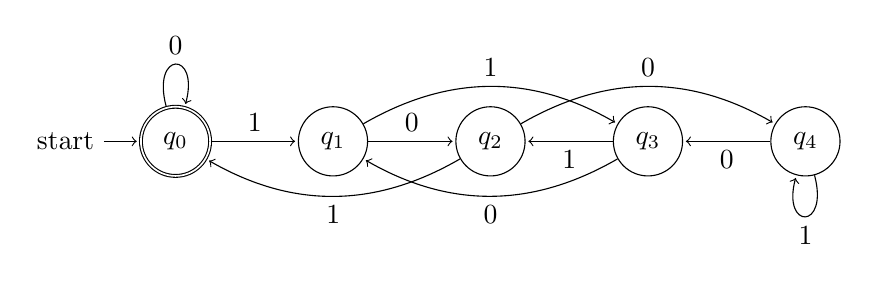
\begin{tikzpicture}[shorten >=1pt,node distance=2cm,on grid,auto] 
            \node[state, accepting, initial] (q_0)   {$q_0$}; 
            \node[state] (q_1) [right=of q_0] {$q_1$}; 
            \node[state] (q_2) [right=of q_1] {$q_2$}; 
            \node[state] (q_3) [right=of q_2] {$q_3$}; 
            \node[state] (q_4) [right=of q_3] {$q_4$}; 
            \path[->] 
                (q_0)
                    edge [loop above] node {0} (q_0)
                    edge node {1} (q_1)
                (q_1)
                    edge node {0} (q_2)
                    edge [bend right=-30] node {1} (q_3)
                (q_2)
                    edge [bend left] node {1} (q_0)
                    edge [bend right=-30] node {0} (q_4)
                (q_3)
                    edge node {1} (q_2)
                    edge [bend left] node {0} (q_1)
                (q_4)
                    edge node {0} (q_3)
                    edge [loop below] node {1} (q_4);
        \end{tikzpicture}
        \caption{DFA, \(A\)}
        \label{fig:automataA}
    \end{figure}

    \textbf{Justification}
    \\

    Take a given binary number, \(x\). Since there are only two inputs to our
    state machine, \(x\) can either become \(x0\) or \(x1\). When a 0 comes into
    the state machine, it is the same as taking the binary number and
    multiplying it by two. When a 1 comes into the machine, it is the same as
    multipying by two and adding one.
    \\

    Using this knowledge, we can construct a transition table that tell us where
    to go:

    \begin{table}[ht]
        \centering
        \begin{tabular}{c || c | c | c | c | c}
             & \(x \mod 5 = 0\) & \(x \mod 5 = 1\) & \(x \mod 5 = 2\) & \(x \mod 5 = 3\) & \(x \mod 5 = 4\) \\
            \hline
            \(x0\) & 0 & 2 & 4 & 1 & 3 \\
            \(x1\) & 1 & 3 & 0 & 2 & 4 \\
        \end{tabular}
    \end{table}

    Therefore on state \(q_0\) or (\(x \mod 5 = 0\)), a transition line should go
    to state \(q_0\) for the input 0 and a line should go to state \(q_1\) for
    input 1. Continuing this gives us the Figure ~\ref{fig:automataA}.

\end{homeworkProblem}

\pagebreak

\begin{homeworkProblem}

\end{homeworkProblem}

\end{document}
